\documentclass[11pt]{article}

\usepackage[utf8]{inputenc}
\usepackage[T1]{fontenc}
\usepackage{lmodern}
\usepackage{microtype}
\usepackage{amsmath}
\usepackage{amssymb}
\usepackage{booktabs}
\usepackage{siunitx}
\usepackage{graphicx}
\usepackage{tikz}
\usepackage{pgfplots}
\usepackage{longtable}
\usepackage{hyperref}
\usepackage{url}
\usepackage{enumitem}
\usepackage{geometry}
\geometry{margin=1in}
\usetikzlibrary{arrows.meta,positioning}
\pgfplotsset{compat=1.18}

\hypersetup{
    colorlinks=true,
    linkcolor=blue,
    citecolor=blue,
    urlcolor=blue
}

\sisetup{
    detect-all=true,
    group-separator={,},
    group-minimum-digits=4
}

\title{kiwi-rs: Ergonomic and Performance-Oriented Rust Bindings\\for the Kiwi Korean Morphological Analyzer}

% Replace with final author metadata before submission.
\author{
Jai-Chang Park
}
\date{February 17, 2026}

\begin{document}
\maketitle

\begin{abstract}
This report presents \texttt{kiwi-rs}, a Rust library that exposes the public Kiwi C API through a high-level and safety-oriented interface for Korean NLP. The implementation combines dynamic symbol loading, ownership-safe handle wrappers, runtime capability checks, and auto-bootstrap for library/model assets, and it includes an agent-skill package for reliable LLM-assisted onboarding. We evaluate \texttt{kiwi-rs} against \texttt{kiwipiepy} under matched conditions using repeated-input (warm-cache) and varied-input (cache-active, mixed-reuse) workloads with bootstrap confidence intervals and sink-parity checks. On a dataset of 192 Korean texts across 8 categories, \texttt{kiwi-rs} shows measurable speedups on selected varied-input features (e.g., \texttt{join}: \(3.85\times\), \texttt{tokenize\_many\_batch}: \(23.18\times\), \texttt{split\_into\_sents\_with\_tokens}: \(67.75\times\)) while other paths remain close to parity or statistically inconclusive under conservative decision rules. Repeated-input numbers are reported as warm-cache capacity bounds only. We additionally report cache-minimized stress results and path-pinned reproducibility runs to bound interpretation of headline ratios.
\end{abstract}

\section{Introduction}
Rust adoption in production NLP systems has increased due to predictable performance, explicit ownership semantics, and strong tooling~\cite{rust_lang}. However, high-quality language analyzers are often distributed as C/C++ runtimes with Python-first interfaces~\cite{kiwi_repo,kiwipiepy}. This creates a practical gap: teams that build Rust services need bindings that are more than thin FFI wrappers.

\subsection{Rust Language Context}
Rust is a systems programming language designed for high performance and memory safety without a garbage collector~\cite{rust_lang}. For NLP service engineering, this combination has practical consequences:
\begin{itemize}[leftmargin=1.5em]
    \item \textbf{Safety at FFI boundaries.} Ownership/borrowing and typed error channels reduce common C interop failure classes (dangling pointers, double free, unchecked null paths).
    \item \textbf{Predictable runtime cost.} Ahead-of-time compilation and zero-cost abstractions fit latency-sensitive inference pipelines.
    \item \textbf{Deployment alignment.} Static binary workflows and mature package tooling (\texttt{cargo}) simplify service shipping and CI integration.
\end{itemize}

In short, Rust is a strong fit when the core analyzer is implemented natively (C/C++) but production orchestration requires safer and more ergonomic application-level APIs.

Existing Rust interop stacks (e.g., generated C bindings, C++ bridge layers, Python bridge toolchains) provide useful foundations~\cite{rust_bindgen,cxx_rs,pyo3}. \texttt{kiwi-rs} is positioned as an engineering-focused integration package on top of those fundamentals: it emphasizes runtime capability detection, deployment bootstrap behavior, and benchmark artifacts rather than proposing a new FFI theory.

\texttt{kiwi-rs} addresses this gap for Kiwi, a Korean morphological analyzer, by providing:
\begin{itemize}[leftmargin=1.5em]
    \item idiomatic Rust APIs for common analysis pipelines;
    \item explicit and safe ownership around FFI handles;
    \item runtime compatibility checks for optional C API surfaces;
    \item reproducible benchmarking utilities for Rust-vs-Python comparison.
\end{itemize}

This document is intentionally an \textbf{engineering technical report}: it prioritizes implementation transparency, reproducibility artifacts, and operational trade-offs over algorithmic novelty claims.

\section{Background: Kiwi}
Kiwi is a Korean morphological analyzer implemented in C++ and distributed with a public C API, which makes it usable across multiple language runtimes~\cite{kiwi_repo}. In practice, Kiwi is commonly consumed through \texttt{kiwipiepy} in Python workflows, while additional ecosystem bindings target other environments~\cite{kiwipiepy,kiwi_repo}.

\subsection{Ecosystem and Distribution Survey}
Upstream Kiwi documentation describes a broad multi-language ecosystem centered on the C API and release-packaged binaries~\cite{kiwi_repo,kiwi_releases,kiwi_gui}. Table~\ref{tab:kiwi_ecosystem} summarizes the currently documented channels and wrappers relevant to market and adoption analysis.

\begin{table}[t]
\centering
\caption{Documented Kiwi ecosystem channels and wrappers (upstream snapshot).}
\label{tab:kiwi_ecosystem}
\begin{tabular}{p{0.30\linewidth}p{0.60\linewidth}}
\toprule
Channel & Notes \\
\midrule
C API & Public header (\texttt{include/kiwi/capi.h}) as primary native integration boundary. \\
Compiled binaries & Release artifacts for Windows, Linux, macOS, and Android (library + model files). \\
C\# wrappers & Official GUI wrapper (\texttt{kiwi-gui}) and community wrapper (\texttt{NetKiwi}). \\
Python wrapper & \texttt{kiwipiepy} as the de facto Python API in production/data workflows. \\
Java wrapper & \texttt{KiwiJava} (Java 1.8+) via \texttt{bindings/java}. \\
Android library & NDK-based AAR distribution (\texttt{kiwi-android-VERSION.aar}); documented minimum Android API level 21+ and ARM64 target. \\
R wrapper & Community wrapper \texttt{elbird}. \\
Go wrapper & Community wrapper \texttt{kiwigo}. \\
WebAssembly & Community JavaScript/TypeScript binding via \texttt{bindings/wasm}. \\
End-user GUI application & Windows-oriented GUI distribution for non-programmer use cases (\texttt{kiwi-gui}). \\
\bottomrule
\end{tabular}
\end{table}

This ecosystem breadth suggests that Kiwi demand spans research scripting, server backends, mobile integration, browser runtimes, and non-programmer desktop tooling. From a market-positioning perspective, \texttt{kiwi-rs} fills the Rust-native integration slot in this existing multi-language stack rather than competing with upstream analyzers or language-specific wrappers.

\subsection{POS Tag Inventory}
Kiwi uses a Sejong-based POS scheme with selected extensions and refinements (e.g., web entities, symbol structure, user-defined categories)~\cite{kiwi_repo}. This is practically important for \texttt{kiwi-rs}, because many downstream integrations consume \texttt{Token.tag} and \texttt{tag\_to\_string} outputs as stable labels.

\begin{table}[t]
\centering
\caption{POS tag groups used by Kiwi (summary).}
\label{tab:pos_summary}
\begin{tabular}{p{0.24\linewidth}p{0.68\linewidth}}
\toprule
Group & Representative Tags \\
\midrule
Nouns and nominals & \texttt{NNG}, \texttt{NNP}, \texttt{NNB}, \texttt{NR}, \texttt{NP} \\
Predicates & \texttt{VV}, \texttt{VA}, \texttt{VX}, \texttt{VCP}, \texttt{VCN} \\
Modifiers and particles & \texttt{MM}, \texttt{MAG}, \texttt{MAJ}, \texttt{IC}, \texttt{JKS}--\texttt{JC} \\
Endings and derivation & \texttt{EP}, \texttt{EF}, \texttt{EC}, \texttt{ETN}, \texttt{ETM}, \texttt{XPN}, \texttt{XSN}, \texttt{XSV}, \texttt{XSA}, \texttt{XSM}, \texttt{XR} \\
Symbols and scripts & \texttt{SF}, \texttt{SP}, \texttt{SS}, \texttt{SSO}, \texttt{SSC}, \texttt{SE}, \texttt{SO}, \texttt{SW}, \texttt{SL}, \texttt{SH}, \texttt{SN}, \texttt{SB} \\
Web and special tags & \texttt{UN}, \texttt{W\_URL}, \texttt{W\_EMAIL}, \texttt{W\_HASHTAG}, \texttt{W\_MENTION}, \texttt{W\_SERIAL}, \texttt{W\_EMOJI}, \texttt{Z\_CODA}, \texttt{Z\_SIOT}, \texttt{USER0}--\texttt{USER4} \\
\bottomrule
\end{tabular}
\end{table}

A full tag-by-tag inventory is provided in Appendix~\ref{app:pos_inventory}, including explicit marking of Kiwi-specific extensions relative to baseline Sejong tags.

\begin{table}[t]
\centering
\caption{Kiwi-specific POS extensions relative to baseline Sejong tags.}
\label{tab:pos_extensions}
\begin{tabular}{p{0.30\linewidth}p{0.60\linewidth}}
\toprule
Extension family & Tags and intent \\
\midrule
Derivation and symbol refinement & \texttt{XSM}, \texttt{SSO}, \texttt{SSC}, \texttt{SB} for finer derivational and symbol-structure distinctions. \\
Unanalyzable and web entities & \texttt{UN}, \texttt{W\_URL}, \texttt{W\_EMAIL}, \texttt{W\_HASHTAG}, \texttt{W\_MENTION}, \texttt{W\_SERIAL}, \texttt{W\_EMOJI}. \\
Orthographic and user channels & \texttt{Z\_CODA}, \texttt{Z\_SIOT}, \texttt{USER0}--\texttt{USER4}. \\
\bottomrule
\end{tabular}
\end{table}

For this work, three Kiwi properties are operationally important:
\begin{itemize}[leftmargin=1.5em]
    \item \textbf{C API boundary.} A stable C-layer contract enables dynamic loading and runtime capability probing from Rust.
    \item \textbf{Release-distributed assets.} Platform libraries and model artifacts are versioned together, allowing explicit compatibility control.
    \item \textbf{Feature breadth.} Kiwi exposes not only core tokenization/analysis but also typo handling, sentence processing, and semantic utilities, enabling a broad Rust wrapper surface.
\end{itemize}

Accordingly, \texttt{kiwi-rs} is designed as a C API-centered integration layer rather than a re-implementation of Kiwi internals. This design choice preserves upstream behavior while focusing engineering effort on safety, ergonomics, and deployment reproducibility.

\section{Scope and Contributions}
As of version \texttt{0.1.4} (snapshot date: 2026-02-17), the project reports complete loader coverage for the published Kiwi C symbols (\(101/101\)) and broad support for high-level workflows in Rust~\cite{kiwi_rs_repo,kiwi_rs_crates}. The crate targets Rust edition 2021 with MSRV 1.70, which supports older production toolchains while keeping modern language ergonomics~\cite{kiwi_rs_repo}. The main contributions are:
\begin{enumerate}[leftmargin=1.5em]
    \item \textbf{A production-oriented Rust surface over Kiwi C API.} The library exposes core and advanced capabilities, including batch APIs, typo models, pretokenization constraints, UTF-16 variants, and semantic CoNg operations (Kiwi context-graph similarity/prediction APIs).
    \item \textbf{A safety-first runtime model.} The implementation uses RAII cleanup (\texttt{Drop}), typed error propagation, runtime feature probing, and internal compatibility guards across object graphs.
    \item \textbf{A practical bootstrap path.} \texttt{Kiwi::init()} can resolve or download matching runtime assets into cache, reducing setup friction while keeping explicit configuration paths available.
    \item \textbf{A reproducible benchmark framework.} The repository includes paired Rust/Python harnesses, repeated and varied input modes, sink parity checks, and bootstrap confidence intervals for defensible speed claims.
    \item \textbf{An agent-skill artifact for developer productivity.} The repository packages an assistant skill that constrains LLM responses to runnable code, explicit initialization choices, one-step validation commands, and request-specific pitfalls.
\end{enumerate}

\section{System Design}
\subsection{Dynamic Loading and Capability Detection}
\texttt{kiwi-rs} loads Kiwi symbols dynamically at runtime and resolves optional APIs when available~\cite{kiwi_rs_repo}. Instead of hard-linking a single ABI assumption, the library checks capability flags (e.g., UTF-16, stream builder init, multi-line UTF-16 analysis support) before exposing optional paths. This design reduces failure modes across heterogeneous deployment environments.

\subsection{Ownership and Handle Safety}
Core runtime objects (library, analyzer, builder, typo model, tokenizer, and intermediate result handles) are wrapped in Rust structs and released via deterministic \texttt{Drop} implementations. Internally shared runtime state uses \texttt{Arc}, while cross-object validity checks prevent accidental mixing of handles originating from different loaded libraries. This avoids a common FFI class of undefined behavior.

\subsection{Error Model}
Public APIs return a typed \texttt{Result<T, KiwiError>} with distinct categories:
\begin{itemize}[leftmargin=1.5em]
    \item \texttt{LibraryLoad}, \texttt{SymbolLoad}, \texttt{NulByte};
    \item \texttt{InvalidArgument}, \texttt{Bootstrap}, \texttt{Api}.
\end{itemize}
This separation improves observability for deployment issues compared to string-only error channels.

\subsection{Initialization Paths}
The library supports three initialization styles:
\begin{enumerate}[leftmargin=1.5em]
    \item \texttt{Kiwi::init()} for auto-bootstrap and cache-based setup;
    \item \texttt{Kiwi::new()} for environment-driven explicit paths;
    \item \texttt{Kiwi::from\_config(...)} for fully controlled runtime configuration.
\end{enumerate}

In auto-bootstrap mode, the runtime resolves release metadata, downloads matching archives, and extracts them to an OS-appropriate cache root (or \texttt{KIWI\_RS\_CACHE\_DIR} override).

\subsection{Inference Hot-Path Caching}
The implementation includes lightweight in-process caches for join, tokenize, analyze, split, and glue operations using bounded queues. While this significantly improves repeated-input throughput, the benchmark protocol explicitly separates repeated-input and varied-input runs to prevent cache-inflated claims.

\begin{figure}[t]
\centering
\resizebox{\linewidth}{!}{%
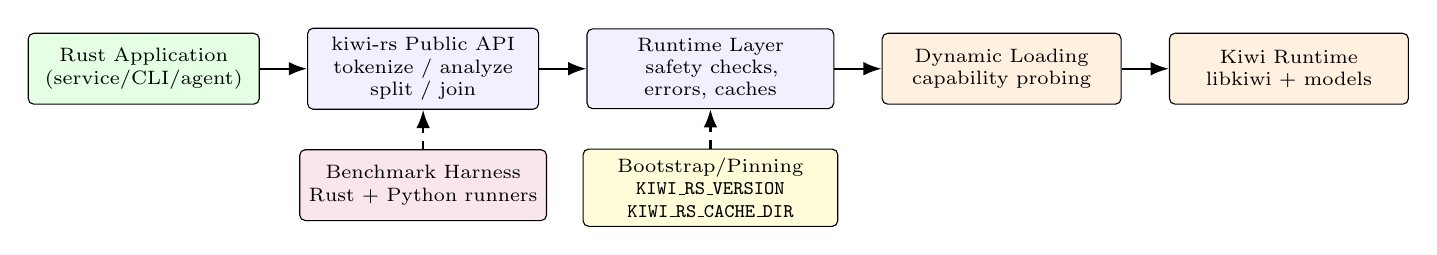
\begin{tikzpicture}[
    box/.style={
        draw,
        rounded corners=2pt,
        align=center,
        font=\scriptsize,
        minimum height=9mm,
        text width=2.7cm,
        fill=blue!6
    },
    edge/.style={-Latex, thick},
    control/.style={-Latex, thick, dashed},
    node distance=5mm and 6mm
]
\node[box, fill=green!10] (app) {Rust Application\\(service/CLI/agent)};
\node[box, right=of app] (api) {kiwi-rs Public API\\tokenize / analyze\\split / join};
\node[box, right=of api, text width=2.9cm] (runtime) {Runtime Layer\\safety checks, errors, caches};
\node[box, right=of runtime, text width=2.8cm, fill=orange!12] (ffi) {Dynamic Loading\\capability probing};
\node[box, right=of ffi, text width=2.8cm, fill=orange!12] (native) {Kiwi Runtime\\libkiwi + models};

\node[box, below=of runtime, text width=3.0cm, fill=yellow!15] (bootstrap) {Bootstrap/Pinning\\\texttt{KIWI\_RS\_VERSION}\\\texttt{KIWI\_RS\_CACHE\_DIR}};
\node[box, below=of api, text width=2.9cm, fill=purple!10] (bench) {Benchmark Harness\\Rust + Python runners};

\draw[edge] (app) -- (api);
\draw[edge] (api) -- (runtime);
\draw[edge] (runtime) -- (ffi);
\draw[edge] (ffi) -- (native);
\draw[control] (bootstrap) -- (runtime);
\draw[control] (bench) -- (api);
\end{tikzpicture}
}
\caption{System architecture of \texttt{kiwi-rs}. Solid arrows show inference flow; dashed arrows show control flow.}
\label{fig:architecture}
\end{figure}

Figure~\ref{fig:architecture} summarizes the practical layering used by the library in production deployments.

\section{Performance Mechanisms}
This section explains \emph{why} the reported throughput numbers can become large on specific features.

\subsection{Recency Caches and Key Design}
\texttt{kiwi-rs} uses bounded recency caches on multiple paths. Cache hits are promoted and old entries are evicted from bounded queues, yielding an LRU-like policy with small fixed capacities.

\begin{table}[t]
\centering
\caption{Primary in-process caches in \texttt{kiwi-rs}.}
\label{tab:cache_design}
\begin{tabular}{lrl}
\toprule
Cache & Capacity & Key Sketch \\
\midrule
\texttt{join\_cache} & 16 & morph sequence + \texttt{lm\_search} \\
\texttt{tokenize\_cache} & 256 & tokenize options + text fingerprint + text equality \\
\texttt{analyze\_cache} & 128 & analyze options + text fingerprint + text equality \\
\texttt{split\_cache} & 64 & \texttt{match\_options} + text fingerprint + text equality \\
\texttt{glue\_cache} & 64 & chunk list + newline flags + glue fingerprint \\
\texttt{glue\_pair\_cache} & 256 & adjacent pair (\texttt{left}, \texttt{right}) \\
\bottomrule
\end{tabular}
\end{table}

Tokenize/analyze/split entries include a compact text fingerprint (length + edge bytes) and then verify full text equality for collision safety. This reduces average key-comparison cost while preserving correctness.

\subsection{Hot-Path Specialization}
Several implementations reduce overhead beyond basic caching:
\begin{itemize}[leftmargin=1.5em]
    \item \textbf{Top-1 fast paths.} Cache-backed analyze/tokenize paths are specialized for \texttt{top\_n=1}, the dominant inference mode in production routing.
    \item \textbf{Joiner reuse APIs.} \texttt{prepare\_join\_morphs} and \texttt{prepare\_joiner} avoid repeated \texttt{CString} construction and joiner re-initialization, which explains large gains in join-heavy microbenchmarks.
    \item \textbf{Glue pair scoring via native batch callback.} \texttt{glue\_with\_options} scores only unresolved adjacent pairs using a native multi-text scoring path, then memoizes pair decisions.
    \item \textbf{Sentence structure construction from token metadata.} This path builds sentence structures directly from token metadata after tokenization, avoiding an extra native split pass.
\end{itemize}

\subsection{Cache Coherence and Safety Trade-offs}
To prevent stale inference outputs after runtime mutation, option/config updates clear inference caches. This favors correctness but can reduce throughput in workloads that frequently change analyzer settings.

\subsection{Implications for Repeated vs Varied Benchmarks}
The large repeated-input speedups are expected from recency caches and prepared-join reuse. For varied-input runs, cache effects can still appear when the active text pool fits cache capacity (e.g., a 192-text pool versus 256-entry tokenize cache). Therefore, very large ratios on some features should be interpreted as \emph{pipeline-aware upper bounds under this harness design}, not universal constants.

\section{API Coverage and Parity Boundaries}
\texttt{kiwi-rs} covers most C API-backed flows and exposes them with Rust-first signatures. Table~\ref{tab:api_surface} summarizes the currently supported API surface by subsystem.

\begin{table}[t]
\centering
\caption{Supported API surface in \texttt{kiwi-rs} (representative groups).}
\label{tab:api_surface}
\begin{tabular}{p{0.30\linewidth}p{0.58\linewidth}}
\toprule
Area & Representative APIs \\
\midrule
Initialization and setup & \texttt{Kiwi::init}, \texttt{Kiwi::new}, \texttt{Kiwi::from\_config}, \texttt{Kiwi::init\_direct} \\
Core inference & \texttt{analyze*}, \texttt{tokenize*}, \texttt{split\_into\_sents*}, \texttt{space*}, \texttt{glue*}, \texttt{join*} \\
Batch and native paths & \texttt{analyze\_many\_with\_options}, \texttt{analyze\_many\_via\_native}, \texttt{tokenize\_many}, \texttt{tokenize\_many\_with\_echo} \\
Builder and lexicon customization & \texttt{add\_user\_word}, \texttt{add\_pre\_analyzed\_word}, \texttt{load\_user\_dictionary}, \texttt{add\_rule}, \texttt{add\_re\_rule}, \texttt{extract\_words*} \\
Constraint and typo models & \texttt{MorphemeSet}, \texttt{Pretokenized}, \texttt{KiwiTypo}, default typo presets \\
Extended APIs & \texttt{SwTokenizer}, CoNg similarity/prediction APIs, UTF-16 variants with runtime support checks \\
\bottomrule
\end{tabular}
\end{table}

At the C API layer, symbol loading coverage is complete (\(101/101\) loader entries at the reported snapshot). For \texttt{kiwipiepy}-surface parity tracking, the current matrix reports 12 \texttt{Equivalent}, 19 \texttt{Partial}, and 9 \texttt{Unavailable} rows (total 40 tracked rows). Full parity is therefore intentionally partial: several Python/C++-specific surfaces (e.g., template layer, dataset/training helpers beyond C API, some utility classes) remain out of scope~\cite{kiwipiepy,kiwi_repo,kiwi_rs_repo}.

\subsection{Agent Skill for LLM-Assisted Usage}
To reduce prompt ambiguity in AI-assisted development, \texttt{kiwi-rs} includes a local skill package (\texttt{skills/kiwi-rs-assistant/}) with:
\begin{itemize}[leftmargin=1.5em]
    \item a structured workflow that routes user intent to API families (tokenize/analyze/split/join, builder, typo, UTF-16, batch, and semantics);
    \item explicit initialization path rules (\texttt{Kiwi::init}, \texttt{Kiwi::new}, \texttt{Kiwi::from\_config}, or builder flow);
    \item a response contract requiring runnable Rust code, a concrete verification command, and request-specific pitfalls;
    \item troubleshooting and parity guardrails that map common errors to concrete fixes and prevent unsupported parity claims.
\end{itemize}

This skill packaging is not presented as a model-quality contribution; instead, it is a reproducible developer-facing artifact that can improve consistency of generated integration code.

\section{Evaluation Methodology}
\subsection{Benchmark Design}
The benchmark protocol compares \texttt{kiwi-rs} and \texttt{kiwipiepy} under aligned settings:
\begin{itemize}[leftmargin=1.5em]
    \item same text workload and dataset source;
    \item same warmup/iteration schedules;
    \item alternating engine order to reduce order bias;
    \item sink parity checks to validate workload equivalence;
    \item bootstrap confidence intervals (95\%) and \(P(\text{ratio}>1)\).
\end{itemize}

Decision thresholds follow a practical equivalence band of \(\pm 5\%\) around parity. For ratio CI \([L, U]\):
\begin{itemize}[leftmargin=1.5em]
    \item \textbf{kiwi-rs faster (robust)} if \(L > 1.05\);
    \item \textbf{kiwipiepy faster (robust)} if \(U < 0.95\);
    \item \textbf{practically equivalent} if \(L \ge 0.95\) and \(U \le 1.05\);
    \item \textbf{kiwi-rs likely faster} if \(L > 1.00\) and not robust;
    \item \textbf{kiwipiepy likely faster} if \(U < 1.00\) and not robust;
    \item \textbf{inconclusive} otherwise.
\end{itemize}

\subsection{Functional Equivalence Scope}
Because this is an engineering report about a binding layer, we separate two notions of equivalence:
\begin{itemize}[leftmargin=1.5em]
    \item \textbf{Workload equivalence} for benchmark fairness, validated by sink parity checks in the harness.
    \item \textbf{API-surface equivalence} against \texttt{kiwipiepy}, tracked in a maintained parity matrix (\(12\) Equivalent, \(19\) Partial, \(9\) Unavailable; total \(40\) rows)~\cite{kiwi_rs_parity_doc}.
\end{itemize}

In addition, integration tests exercise representative end-to-end behaviors (\texttt{tokenize}, \texttt{analyze}, sentence splitting, spacing, joining, and user-word injection) to catch regressions in practical outputs~\cite{kiwi_rs_repo}. We do not claim corpus-level linguistic accuracy gains over upstream Kiwi in this paper; the focus is wrapper behavior and performance.

\subsection{Cross-Engine Agreement Protocol}
To complement throughput measurements with NLP-relevant structural checks, we added a cross-engine agreement protocol on the same 192-text dataset. This protocol compares \texttt{kiwi-rs} against \texttt{kiwipiepy} for:
\begin{itemize}[leftmargin=1.5em]
    \item exact token-sequence agreement (form, POS tag, start, end);
    \item token-boundary set agreement (precision/recall/F1 on spans);
    \item token set agreement (span + form + POS tag precision/recall/F1);
    \item POS agreement rate on shared spans;
    \item sentence-boundary exact agreement.
\end{itemize}

The implementation uses a two-step reproducible path:
\begin{enumerate}[leftmargin=1.5em]
    \item dump \texttt{kiwi-rs} structural outputs via \path{examples/dump_structural_outputs.rs};
    \item compare those outputs against \texttt{kiwipiepy} via \path{scripts/compare_structural_parity.py}.
\end{enumerate}
Sentence boundaries are normalized to character offsets for cross-engine comparability because some Kiwi C-level paths expose byte-indexed boundaries.

\subsection{Dataset and Environment}
The dataset benchmark uses \texttt{benchmarks/datasets/swe\_textset\_v2.tsv}:
\begin{itemize}[leftmargin=1.5em]
    \item 192 rows, 192 unique texts, 8 categories;
    \item SHA-256: \texttt{8c81b8e8d0c4272f96c05e6851da10759f02361caa0a2acb881dd72e642f4696};
    \item text length (characters): min 14, median 63, max 192.
\end{itemize}

Reported runs were executed on a local development host, Rust 1.93.1, Python 3.14.3, and \texttt{kiwipiepy} 0.22.2, with \(5\) repeats and \(2000\) bootstrap samples.

\subsection{Runtime Pinning and Artifact Lock}
Captured benchmark artifacts include explicit environment snapshots. We use two reporting tiers:
\begin{itemize}[leftmargin=1.5em]
    \item \textbf{Tier A (cache-active baseline, main tables).} Dataset-based varied/repeated runs with auto-discovery (\texttt{KIWI\_LIBRARY\_PATH}, \texttt{KIWI\_MODEL\_PATH} unset).
    \item \textbf{Tier B (path-pinned reproducibility run).} Explicit pinning with:
    \begin{itemize}[leftmargin=1.2em]
        \item \texttt{KIWI\_LIBRARY\_PATH=<KIWI\_LIB\_PATH>}
        \item \texttt{KIWI\_MODEL\_PATH=<KIWI\_MODEL\_DIR>}
        \item \texttt{--python-model-path <KIWI\_MODEL\_DIR>}
    \end{itemize}
\end{itemize}

For Tier A primary runs, the harness recorded:
\begin{itemize}[leftmargin=1.5em]
    \item \texttt{Git SHA}: \texttt{<REPO\_COMMIT\_SHA>} (\texttt{dirty=<true|false>});
    \item \texttt{KIWI\_LIBRARY\_PATH}: unset;
    \item \texttt{KIWI\_MODEL\_PATH}: unset.
\end{itemize}

Given this configuration, the runtime was resolved by \texttt{Kiwi::init()} fallback logic at execution time. Therefore, Tier A artifacts are reproducible at the harness level but not immutable to future upstream release drift unless explicit pinning is used~\cite{kiwi_rs_repo}.

For Tier B, we additionally recorded hash-anchored assets:
\begin{itemize}[leftmargin=1.5em]
    \item \texttt{libkiwi.0.22.2.dylib}: \texttt{e541f158 62e26a44 50f7b0b1 b2355978}\\
    \hspace*{2.2em}\texttt{c8e498e9 73f9c917 783f2350 81b54bce};
    \item \texttt{cong.mdl}: \texttt{bd9ca89e e1b72e75 0c8e2166 a17c80a0}\\
    \hspace*{2.2em}\texttt{fe3fabd8 28c78b1f 0928486a 6b1833a7};
    \item \texttt{sj.morph}: \texttt{5e3dab2d ef6d2cc0 79e21d54 77bd610a}\\
    \hspace*{2.2em}\texttt{391c6904 5d08caf1 e0bbeabd a8db8d1b};
    \item \texttt{default.dict}: \texttt{d4293e44 b2588d0c 3aabbce6 07a0f41a}\\
    \hspace*{2.2em}\texttt{d3534abd 31b34139 847b1272 54e01549}.
\end{itemize}

We note one remaining boundary for strict cross-engine identity: \texttt{kiwipiepy} uses its packaged native extension, so exact binary identity with the Rust-side dynamically loaded \texttt{libkiwi} cannot be guaranteed in this harness even when model paths are pinned.

\subsection{Test Coverage Measurement}
We additionally measured Rust test coverage with \texttt{cargo llvm-cov} to report test adequacy in a reproducible form. Coverage was measured using:
\begin{itemize}[leftmargin=1.5em]
    \item full workspace profile:
    \begin{quote}
    \small\texttt{cargo llvm-cov --workspace --summary-only}\\
    \small\texttt{-- --skip test\_add\_rule\_safety}
    \end{quote}
    \item core-logic profile (excluding FFI boundary-heavy wrappers):
    \begin{quote}
    \small\texttt{cargo llvm-cov --workspace --summary-only}\\
    \small\texttt{--ignore-filename-regex 'runtime\textbackslash{}.rs|native\textbackslash{}.rs'}\\
    \small\texttt{-- --skip test\_add\_rule\_safety}
    \end{quote}
\end{itemize}

The second profile is included because this project contains a large volume of thin FFI wrapper code (\texttt{runtime.rs}, \texttt{native.rs}) whose branch space is dominated by external-library state and optional symbol availability. Concretely, these two files account for 6603/9077 lines (\(72.75\%\)) of \texttt{src/} lines in the measured snapshot. Table~\ref{tab:coverage_profiles} summarizes the resulting coverage.

\begin{table}[t]
\centering
\caption{Coverage summary from \texttt{cargo llvm-cov} (workspace tests).}
\label{tab:coverage_profiles}
\begin{tabular}{lccc}
\toprule
Profile & Region Cover & Line Cover & Function Cover \\
\midrule
Full workspace & 43.02\% & 41.12\% & 47.45\% \\
Core logic (excluding \texttt{runtime.rs}/\texttt{native.rs}) & 94.69\% & 92.84\% & 94.21\% \\
\bottomrule
\end{tabular}
\end{table}

In this paper, when we refer to ``core-logic line coverage \(>90\%\)'', we mean the filtered profile above, not the unfiltered full-wrapper profile.

\section{Results}
\subsection{Varied-Input (Cache-Active) Results}
Table~\ref{tab:varied} reports representative features from the dataset-based varied-input profile. This profile should be read as \emph{cache-active mixed-reuse}, not cache-free: the 192-entry text pool can still interact with bounded caches and warm paths. Clear gains appear in \texttt{join}, \texttt{tokenize\_many\_batch}, and \texttt{split\_into\_sents\_with\_tokens}. Other features remain near parity or inconclusive under the strict decision rule.

\begin{table}[t]
\centering
\caption{Selected throughput ratios on cache-active varied-input profile (\texttt{kiwi-rs} / \texttt{kiwipiepy}).}
\label{tab:varied}
\begin{tabular}{lcccc}
\toprule
Feature & Ratio & 95\% CI & \(P(\text{ratio}>1)\) & Decision \\
\midrule
\texttt{tokenize} & 1.49x & [0.97, 1.55] & 0.955 & inconclusive \\
\texttt{split\_into\_sents} & 1.06x & [1.02, 1.12] & 1.000 & likely faster \\
\texttt{split\_into\_sents\_with\_tokens} & 67.75x & [63.09, 69.85] & 1.000 & robust faster \\
\texttt{space} & 1.12x & [1.05, 1.21] & 1.000 & likely faster \\
\texttt{join} & 3.85x & [3.68, 4.40] & 1.000 & robust faster \\
\texttt{glue} & 1.56x & [1.43, 1.68] & 1.000 & robust faster \\
\texttt{analyze\_many\_native} & 0.92x & [0.70, 1.00] & 0.029 & inconclusive \\
\texttt{tokenize\_many\_batch} & 23.18x & [21.05, 23.59] & 1.000 & robust faster \\
\texttt{space\_many\_batch} & 0.98x & [0.89, 1.47] & 0.340 & inconclusive \\
\bottomrule
\end{tabular}
\end{table}

\begin{figure}[t]
\centering
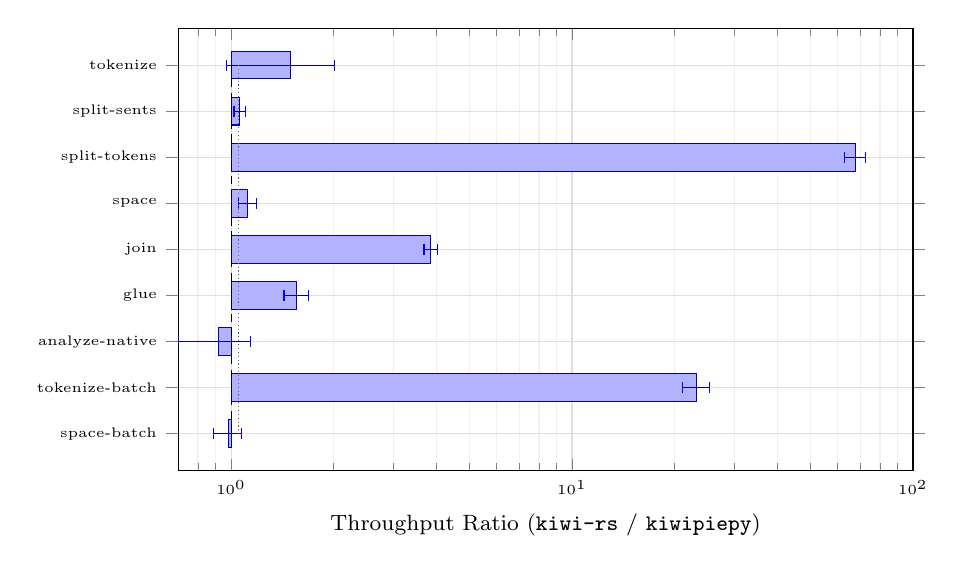
\begin{tikzpicture}
\begin{axis}[
    xbar,
    width=0.90\linewidth,
    height=7.2cm,
    xmode=log,
    xmin=0.7,
    xmax=100,
    xlabel={Throughput Ratio (\texttt{kiwi-rs} / \texttt{kiwipiepy})},
    symbolic y coords={tok,split,splittok,space,join,glue,anative,tokbatch,spacebatch},
    ytick=data,
    yticklabels={
        tokenize,
        split-sents,
        split-tokens,
        space,
        join,
        glue,
        analyze-native,
        tokenize-batch,
        space-batch
    },
    y dir=reverse,
    grid=both,
    major grid style={gray!25},
    minor grid style={gray!12},
    tick label style={font=\tiny},
    label style={font=\footnotesize}
]
\addplot+[
    draw=blue!70!black,
    fill=blue!30,
    xbar,
    error bars/.cd,
    x dir=both,
    x explicit
] coordinates {
    (1.49,tok) +- (0.52,0.06)
    (1.06,split) +- (0.04,0.06)
    (67.75,splittok) +- (4.66,2.10)
    (1.12,space) +- (0.07,0.09)
    (3.85,join) +- (0.17,0.55)
    (1.56,glue) +- (0.13,0.12)
    (0.92,anative) +- (0.22,0.08)
    (23.18,tokbatch) +- (2.13,0.41)
    (0.98,spacebatch) +- (0.09,0.49)
};
\draw[black, densely dashed] (axis cs:1,tok) -- (axis cs:1,spacebatch);
\draw[black!60, densely dotted] (axis cs:1.05,tok) -- (axis cs:1.05,spacebatch);
\end{axis}
\end{tikzpicture}
\caption{Varied-input throughput ratios with 95\% bootstrap confidence intervals. Dashed: parity (\(1.0\times\)); dotted: practical threshold (\(1.05\times\)). Feature labels are abbreviated for readability.}
\label{fig:varied_ci}
\end{figure}

All listed features passed sink parity checks (\(1.0000\times\) ratio), indicating equivalent measured workloads between engines for the compared runs.
Figure~\ref{fig:varied_ci} provides a visual summary of the varied-input outcomes and uncertainty ranges.

\subsection{Cache-Minimized Stress Profile}
To isolate cache effects, we ran an additional synthetic varied-input stress profile with a large variant pool (\texttt{variant\_pool=65536}, no dataset TSV). Under this setting, repeated reuse is strongly reduced for both single-text and batch paths. Table~\ref{tab:cache_minimized} summarizes representative outcomes.

\begin{table}[t]
\centering
\caption{Representative ratios under cache-minimized synthetic stress profile (\texttt{kiwi-rs} / \texttt{kiwipiepy}, 5 repeats).}
\label{tab:cache_minimized}
\begin{tabular}{lccc}
\toprule
Feature & Ratio & 95\% CI & Decision \\
\midrule
\texttt{tokenize} & 1.00x & [0.91, 1.70] & inconclusive \\
\texttt{split\_into\_sents\_with\_tokens} & 0.99x & [0.90, 1.17] & inconclusive \\
\texttt{space} & 1.09x & [0.75, 1.36] & inconclusive \\
\texttt{join} & 5.25x & [4.65, 6.81] & kiwi-rs faster (robust) \\
\texttt{analyze\_many\_native} & 0.91x & [0.69, 1.01] & inconclusive \\
\texttt{tokenize\_many\_batch} & 0.88x & [0.77, 2.82] & inconclusive \\
\bottomrule
\end{tabular}
\end{table}

Compared to Table~\ref{tab:varied}, this stress profile shows that several large dataset-varied gains are strongly cache- and pipeline-dependent. The consistently robust gain in this stress setup is \texttt{join}, while most other features become statistically inconclusive.

\subsection{Path-Pinned Dataset Run}
Under Tier B path pinning (\texttt{KIWI\_LIBRARY\_PATH}, \texttt{KIWI\_MODEL\_PATH}, and \texttt{--python-model-path} all set to explicit local paths), key directional outcomes remain similar. Table~\ref{tab:pinned_selected} reports representative ratios.

\begin{table}[t]
\centering
\caption{Selected outcomes on path-pinned dataset varied-input run (\texttt{kiwi-rs} / \texttt{kiwipiepy}, 5 repeats).}
\label{tab:pinned_selected}
\begin{tabular}{lccc}
\toprule
Feature & Ratio & 95\% CI & Decision \\
\midrule
\texttt{tokenize} & 1.31x & [1.13, 2.30] & kiwi-rs faster (robust) \\
\texttt{split\_into\_sents\_with\_tokens} & 68.38x & [60.25, 107.79] & kiwi-rs faster (robust) \\
\texttt{join} & 3.88x & [3.39, 4.70] & kiwi-rs faster (robust) \\
\texttt{analyze\_many\_native} & 0.93x & [0.81, 1.07] & inconclusive \\
\texttt{tokenize\_many\_batch} & 26.41x & [25.23, 39.38] & kiwi-rs faster (robust) \\
\texttt{space\_many\_batch} & 0.99x & [0.88, 1.13] & inconclusive \\
\bottomrule
\end{tabular}
\end{table}

Startup medians also shift under pinning: unpinned varied-input run shows \(1326.721\) ms (\texttt{kiwi-rs}) vs \(622.918\) ms (\texttt{kiwipiepy}), while path-pinned varied-input run shows \(1461.594\) ms vs \(764.915\) ms (both \(n=5\)). This reinforces that startup comparisons should be interpreted with explicit runtime-path metadata rather than as universal constants.

\subsection{Cross-Engine Structural Agreement}
Table~\ref{tab:agreement_core} summarizes structural agreement between \texttt{kiwi-rs} and \texttt{kiwipiepy} on \path{swe_textset_v2.tsv}. Agreement is high overall. Token-boundary F1 is \(1.0000\), token (span+form+tag) F1 is \(0.9990\), and POS agreement on shared spans is \(99.90\%\).

\begin{table}[t]
\centering
\caption{Cross-engine structural agreement (\texttt{kiwi-rs} vs \texttt{kiwipiepy}, 192 rows).}
\label{tab:agreement_core}
\begin{tabular}{lr}
\toprule
Metric & Value \\
\midrule
Exact token-sequence match rate & \(186/192 = 96.88\%\) \\
Exact sentence-boundary match rate & \(192/192 = 100.00\%\) \\
Token-boundary precision / recall / F1 & \(1.0000 / 1.0000 / 1.0000\) \\
Token (span+form+tag) precision / recall / F1 & \(0.9990 / 0.9990 / 0.9990\) \\
POS agreement on shared spans & \(5858/5864 = 99.90\%\) \\
\bottomrule
\end{tabular}
\end{table}

At row level, sentence and token-boundary mismatches were zero after boundary normalization, while POS mismatches occurred in 6 rows. Table~\ref{tab:agreement_confusions} lists the observed POS confusion pairs.

\begin{table}[t]
\centering
\caption{Observed POS confusion pairs on shared spans (cross-engine comparison).}
\label{tab:agreement_confusions}
\begin{tabular}{lrc}
\toprule
\texttt{kiwi-rs} tag & \texttt{kiwipiepy} tag & Count \\
\midrule
\texttt{VX} & \texttt{VX-R} & 3 \\
\texttt{VV} & \texttt{VV-R} & 3 \\
\bottomrule
\end{tabular}
\end{table}

In this comparison stream, the \texttt{-R} suffix (e.g., \texttt{VV-R}, \texttt{VX-R}) appears on the \texttt{kiwipiepy} side as a tag-variant marker. We treat these as tag-variant disagreements on identical spans, not as boundary mismatches.

These mismatches are concentrated in \texttt{typo\_noisy} and \texttt{longform} categories. They appear as fine-grained tag variant differences (\texttt{VV} vs \texttt{VV-R}, \texttt{VX} vs \texttt{VX-R}) rather than segmentation disagreements. Table~\ref{tab:agreement_category} and Figure~\ref{fig:agreement_category} report exact token-sequence agreement by category.

\begin{table}[t]
\centering
\caption{Exact token-sequence agreement by category.}
\label{tab:agreement_category}
\begin{tabular}{lrr}
\toprule
Category & Matches / Total & Rate \\
\midrule
\texttt{news} & \(24/24\) & \(100.00\%\) \\
\texttt{colloquial} & \(24/24\) & \(100.00\%\) \\
\texttt{code\_mixed} & \(24/24\) & \(100.00\%\) \\
\texttt{ecommerce} & \(24/24\) & \(100.00\%\) \\
\texttt{finance} & \(24/24\) & \(100.00\%\) \\
\texttt{tech} & \(24/24\) & \(100.00\%\) \\
\texttt{typo\_noisy} & \(21/24\) & \(87.50\%\) \\
\texttt{longform} & \(21/24\) & \(87.50\%\) \\
\bottomrule
\end{tabular}
\end{table}

\begin{figure}[t]
\centering
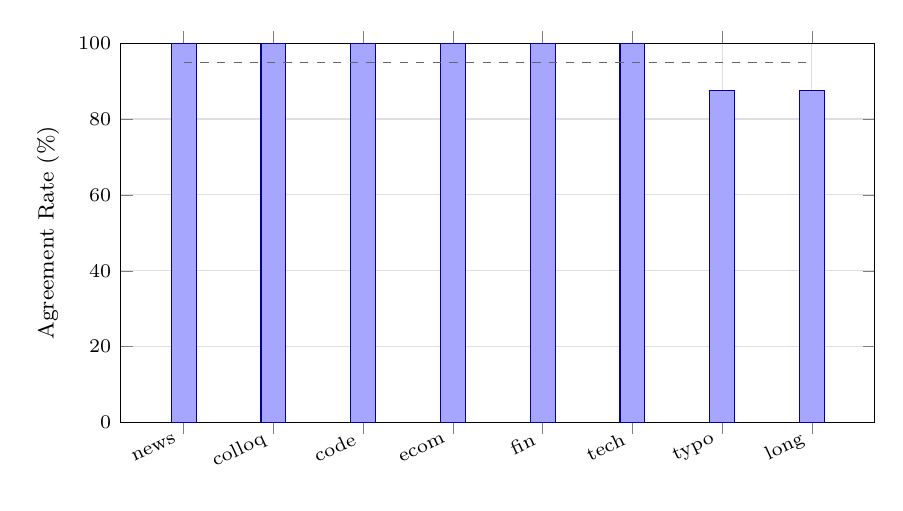
\begin{tikzpicture}
\begin{axis}[
    width=0.92\linewidth,
    height=6.4cm,
    ybar,
    ymin=0,
    ymax=100,
    ylabel={Agreement Rate (\%)},
    symbolic x coords={news,colloq,code,ecom,fin,tech,typo,long},
    xtick=data,
    xticklabel style={font=\scriptsize, rotate=25, anchor=east},
    yticklabel style={font=\scriptsize},
    label style={font=\footnotesize},
    bar width=9pt,
    grid=both,
    major grid style={gray!25},
    minor grid style={gray!12}
]
\addplot+[fill=blue!35, draw=blue!65!black] coordinates {
    (news,100)
    (colloq,100)
    (code,100)
    (ecom,100)
    (fin,100)
    (tech,100)
    (typo,87.5)
    (long,87.5)
};
\draw[black!60, dashed] (axis cs:news,95) -- (axis cs:long,95);
\end{axis}
\end{tikzpicture}
\caption{Category-level exact token-sequence agreement rates (\texttt{kiwi-rs} vs \texttt{kiwipiepy}).}
\label{fig:agreement_category}
\end{figure}

Interpretation should remain conservative: these are cross-engine agreement metrics, not human-annotated linguistic accuracy scores.

\subsection{Repeated-Input (Warm-Cache) Results}
Repeated-input measurements show substantially larger speedups for cache-sensitive paths (e.g., \texttt{tokenize}: \(156.03\times\), \texttt{glue}: \(542.54\times\), \texttt{split\_into\_sents}: \(9445.91\times\)). These values are best interpreted as warm-cache upper bounds, not as default deployment expectations.

\subsection{Category-Stratified Snapshot}
In addition to overall varied-input runs, we used category-stratified evaluation on 8 dataset categories (\texttt{code\_mixed}, \texttt{colloquial}, \texttt{ecommerce}, \texttt{finance}, \texttt{longform}, \texttt{news}, \texttt{tech}, \texttt{typo\_noisy}). Table~\ref{tab:category} summarizes per-category median relative throughput and the weakest feature in each category.
Here, each category's ``Median Ratio'' is the median over the 15 common features, where each feature ratio is computed as:
\[
\mathrm{ratio}_f = \frac{\mathrm{median\ calls/sec}_{\texttt{kiwi-rs},f}}{\mathrm{median\ calls/sec}_{\texttt{kiwipiepy},f}}.
\]

\begin{table}[t]
\centering
\caption{Category-stratified summary (varied input, per-category runs).}
\label{tab:category}
\begin{tabular}{lcc}
\toprule
Category & Median Ratio & Weakest Feature (Ratio) \\
\midrule
\texttt{code\_mixed} & 40.23x & \texttt{join} (4.29x) \\
\texttt{colloquial} & 53.59x & \texttt{join} (3.98x) \\
\texttt{ecommerce} & 53.79x & \texttt{join} (4.27x) \\
\texttt{finance} & 49.18x & \texttt{join} (3.62x) \\
\texttt{longform} & 56.26x & \texttt{join} (4.70x) \\
\texttt{news} & 53.04x & \texttt{join} (3.66x) \\
\texttt{tech} & 43.72x & \texttt{join} (3.12x) \\
\texttt{typo\_noisy} & 70.02x & \texttt{join} (3.97x) \\
\bottomrule
\end{tabular}
\end{table}

These category runs should be interpreted as a complementary robustness signal rather than a direct replacement for the overall varied-input baseline. In particular, category-local text pools can still include repeated forms and may amplify cache effects.

\subsection{Repeated vs Varied Snapshot (All Common Features)}
To provide full cross-mode visibility, Table~\ref{tab:full_snapshot} reports all 15 common benchmark features shared by both engines. This table includes repeated-input and varied-input ratios, plus \(\Delta\%\) relative to parity (\(1.0\times\)).

\begin{table}[t]
\centering
\caption{Full repeated-vs-varied ratio snapshot (\texttt{kiwi-rs} / \texttt{kiwipiepy}) for all common features.}
\label{tab:full_snapshot}
\scriptsize
\resizebox{\linewidth}{!}{%
\begin{tabular}{lrrrr}
\toprule
Feature & Repeated Ratio & Repeated \(\Delta\%\) & Varied Ratio & Varied \(\Delta\%\) \\
\midrule
\texttt{analyze\_many\_loop} & 150.10x & +14909.5\% & 0.96x & -3.9\% \\
\texttt{analyze\_many\_native} & 24.10x & +2309.9\% & 0.92x & -7.9\% \\
\texttt{analyze\_top1} & 148.44x & +14744.4\% & 1.00x & +0.3\% \\
\texttt{batch\_analyze\_native} & 24.10x & +2309.9\% & 0.92x & -7.9\% \\
\texttt{glue} & 542.54x & +54153.8\% & 1.56x & +56.2\% \\
\texttt{join} & 4.30x & +329.9\% & 3.85x & +285.1\% \\
\texttt{space} & 99.02x & +9802.0\% & 1.12x & +11.8\% \\
\texttt{space\_many\_batch} & 14.23x & +1322.6\% & 0.98x & -1.7\% \\
\texttt{space\_many\_loop} & 83.17x & +8217.0\% & 1.05x & +5.0\% \\
\texttt{split\_into\_sents} & 9445.91x & +944491.2\% & 1.06x & +6.4\% \\
\texttt{split\_into\_sents\_with\_tokens} & 86.64x & +8564.1\% & 67.75x & +6675.4\% \\
\texttt{split\_many\_loop} & 1.06x & +6.1\% & 0.92x & -8.3\% \\
\texttt{tokenize} & 156.03x & +15503.4\% & 1.49x & +48.9\% \\
\texttt{tokenize\_many\_batch} & 24.62x & +2362.2\% & 23.18x & +2217.9\% \\
\texttt{tokenize\_many\_loop} & 160.42x & +15942.0\% & 153.21x & +15221.1\% \\
\bottomrule
\end{tabular}%
}
\normalsize
\end{table}

\begin{figure}[t]
\centering
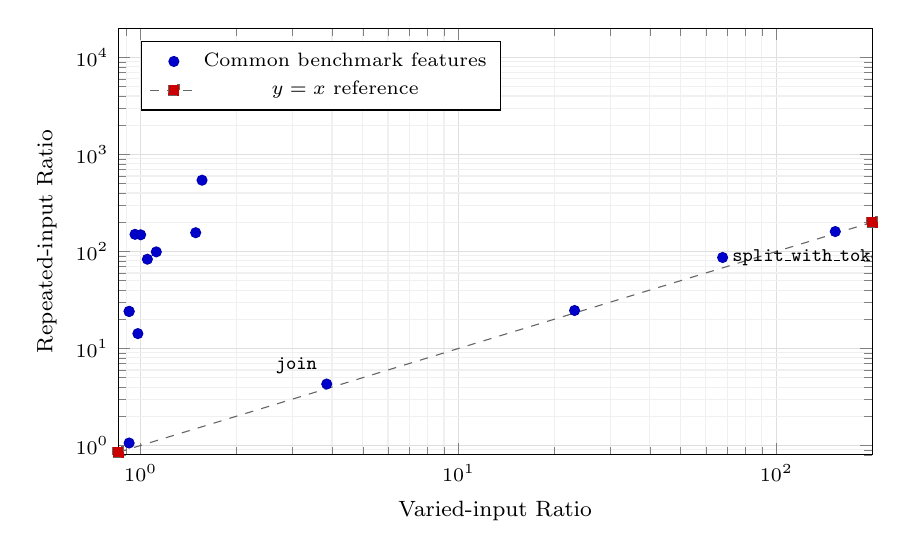
\begin{tikzpicture}
\begin{axis}[
    width=0.92\linewidth,
    height=7.0cm,
    xmode=log,
    ymode=log,
    xmin=0.85,
    xmax=200,
    ymin=0.8,
    ymax=20000,
    xlabel={Varied-input Ratio},
    ylabel={Repeated-input Ratio},
    grid=both,
    major grid style={gray!25},
    minor grid style={gray!12},
    tick label style={font=\scriptsize},
    label style={font=\footnotesize},
    legend pos=north west,
    legend style={font=\scriptsize}
]
\addplot+[
    only marks,
    mark=*,
    mark size=1.8pt,
    color=blue!70!black
] coordinates {
    (0.96,150.10)
    (0.92,24.10)
    (1.00,148.44)
    (0.92,24.10)
    (1.56,542.54)
    (3.85,4.30)
    (1.12,99.02)
    (0.98,14.23)
    (1.05,83.17)
    (1.06,9445.91)
    (67.75,86.64)
    (0.92,1.06)
    (1.49,156.03)
    (23.18,24.62)
    (153.21,160.42)
};
\addlegendentry{Common benchmark features}
\addplot+[domain=0.85:200, samples=2, dashed, color=black!60] {x};
\addlegendentry{$y=x$ reference}
\node[anchor=west, font=\scriptsize] at (axis cs:1.06,9445.91) {\texttt{split\_into\_sents}};
\node[anchor=west, font=\scriptsize] at (axis cs:67.75,86.64) {\texttt{split\_with\_tokens}};
\node[anchor=south east, font=\scriptsize] at (axis cs:3.85,4.30) {\texttt{join}};
\end{axis}
\end{tikzpicture}
\caption{Repeated-input vs varied-input ratio map for all common features. Distance above the \(y=x\) line indicates stronger cache/warm-path amplification.}
\label{fig:repeated_vs_varied}
\end{figure}

Figure~\ref{fig:repeated_vs_varied} highlights that several features are near the diagonal (mode-stable), while others move far upward under repeated-input conditions.

\subsection{Engine-Specific Features}
Table~\ref{tab:engine_specific} reports features not shared between both engines in the current harness (4 Rust-only features and 1 Python-only feature).

\begin{table}[t]
\centering
\caption{Engine-specific benchmark features (median calls/sec).}
\label{tab:engine_specific}
\begin{tabular}{lrr}
\toprule
Feature & Repeated & Varied \\
\midrule
\texttt{join\_prepared} (Rust-only) & 142877.01 & 145837.51 \\
\texttt{join\_prepared\_utf16} (Rust-only) & 149083.73 & 149551.35 \\
\texttt{joiner\_reuse} (Rust-only) & 1841428.46 & 1836727.20 \\
\texttt{joiner\_reuse\_utf16} (Rust-only) & 2289342.35 & 2047194.66 \\
\texttt{split\_many\_batch} (Python-only) & 127.54 & 100.10 \\
\bottomrule
\end{tabular}
\end{table}

\subsection{Startup Cost}
Initialization latency is sensitive to pinning profile and initialization mode. Table~\ref{tab:startup_profiles} reports startup medians and IQRs from measured runs.

\begin{table}[t]
\centering
\caption{Startup latency summary (\texttt{init\_ms}, lower is better).}
\label{tab:startup_profiles}
\begin{tabular}{p{0.34\linewidth}p{0.27\linewidth}p{0.27\linewidth}}
\toprule
Profile & \texttt{kiwi-rs} & \texttt{kiwipiepy} \\
\midrule
Tier A unpinned, dataset-varied (\(n=5\)) & \(1326.721\) ms [Q1 \(1313.006\), Q3 \(1329.406\)] & \(622.918\) ms [Q1 \(618.782\), Q3 \(648.147\)] \\
Tier B path-pinned, dataset-varied (\(n=5\)) & \(1461.594\) ms [Q1 \(1442.657\), Q3 \(1471.654\)] & \(764.915\) ms [Q1 \(686.409\), Q3 \(839.677\)] \\
\bottomrule
\end{tabular}
\end{table}

For Tier A, bootstrap median CIs are \([1278.838, 1474.234]\) ms (\texttt{kiwi-rs}) and \([617.882, 655.605]\) ms (\texttt{kiwipiepy}). We also probed Rust init paths with a lightweight startup-only workload (\(n=5\)): \texttt{Kiwi::init()} median \(1294.165\) ms vs \texttt{Kiwi::new()} median \(1304.267\) ms (no consistent reduction in this setup). Overall, startup is dominated by runtime discovery/loading behavior and should be interpreted with explicit path metadata.

\section{Discussion}
The results suggest two key points:
\begin{enumerate}[leftmargin=1.5em]
    \item \textbf{Steady-state behavior is feature-dependent.} Several operations show strong relative gains, while some batch paths remain near parity.
    \item \textbf{Evaluation mode materially affects interpretation.} Warm-cache runs can overstate general speedups; dataset-varied runs are still cache-active; cache-minimized stress runs provide a stricter bound.
\end{enumerate}

For production systems, this implies a simple policy: report all three modes together (repeated-input, dataset-varied, cache-minimized stress) and use the cache-minimized mode to sanity-check whether large ratios are robust beyond cache/pipeline effects.

\section{Threats to Validity}
\begin{itemize}[leftmargin=1.5em]
    \item \textbf{Single host profile.} Results were collected on one machine and one OS; cross-hardware variance is not yet quantified.
    \item \textbf{Version snapshot effects.} Results depend on specific versions of Kiwi, \texttt{kiwi-rs}, \texttt{kiwipiepy}, Rust, and Python.
    \item \textbf{Cross-engine binary identity boundary.} Even with explicit model-path pinning, \texttt{kiwipiepy}'s packaged native extension limits strict binary-level identity with Rust-side dynamic loading.
    \item \textbf{Cache interactions.} Even varied-input configurations may retain partial repetition, especially in category-constrained pools.
    \item \textbf{Process-level overhead differences.} Language runtime overheads and bridge paths differ between Rust and Python and can affect per-feature behavior.
    \item \textbf{No corpus-level linguistic metric in this report.} We report wrapper parity/behavior and throughput, not task-level morphological accuracy deltas versus upstream Kiwi.
\end{itemize}

\section{Limitations and Future Work}
\begin{itemize}[leftmargin=1.5em]
    \item \textbf{Single-machine benchmark scope.} Current results are from one hardware/OS stack.
    \item \textbf{Startup gap.} \texttt{Kiwi::init()} convenience introduces startup overhead that should be reduced or amortized.
    \item \textbf{Parity gaps.} Python/C++-specific layers remain out of scope under a strict C API binding strategy.
    \item \textbf{Thread-safety assumptions in upstream runtime.} Some test paths are intentionally serialized around initialization due to observed instability in concurrent setup/teardown.
    \item \textbf{Tier-dependent runtime immutability.} Tier B includes explicit binary/model hashes, but the Tier A baseline intentionally uses auto-discovery and is therefore less immutable across future upstream drift.
    \item \textbf{Qualitative ecosystem survey.} Wrapper/channel landscape is documented, but adoption telemetry (downloads, active dependents) is not yet normalized in this report.
\end{itemize}

Planned work includes broader hardware validation, additional memory profiling, startup optimization, immutable runtime lock manifests (release tag + binary/model hashes), and clearly separated optional modules for non-C-API parity features.

\section{Reproducibility Checklist}
For external review, the following should be published with any claim:
\begin{enumerate}[leftmargin=1.5em]
    \item exact benchmark commands and flags;
    \item dataset path and SHA-256 hash;
    \item Rust/Python/package versions;
    \item Git SHA and dirty/clean status;
    \item Kiwi runtime lock (release tag or explicit library/model paths) with binary/model SHA-256 hashes;
    \item varied-input and repeated-input outputs;
    \item ratio CIs, \(P(\text{ratio}>1)\), and sink parity table.
\end{enumerate}

The repository already includes scripts and generated artifacts for this checklist under \path{tmp/feature_dataset_matrix_v2_varied_r5_i300} and related directories.

\section{Conclusion}
\texttt{kiwi-rs} shows that a Rust-first binding over the Kiwi C API can provide practical ergonomics and explicit safety boundaries. The benchmark evidence supports substantial gains for selected features while also highlighting near-parity regions and startup trade-offs. Overall, the library is a practical option for Rust-native Korean NLP services when paired with transparent, workload-aware evaluation.

\section*{Artifact and License Notes}
\texttt{kiwi-rs} is released under LGPL-2.1-or-later. This manuscript reports software benchmark data; it does not contain user-identifying or sensitive human-subject data.

\bibliographystyle{plain}
\bibliography{references}

\appendix
\section{Full POS Tag Inventory}
\label{app:pos_inventory}
\small
\begin{longtable}{p{0.17\linewidth}p{0.14\linewidth}p{0.41\linewidth}p{0.16\linewidth}}
\caption{Kiwi POS tags used in practice (Sejong-based with extensions).} \\
\toprule
Major Group & Tag & Description & Scheme \\
\midrule
\endfirsthead
\toprule
Major Group & Tag & Description & Scheme \\
\midrule
\endhead
\bottomrule
\endfoot
Noun (N) & \texttt{NNG} & common noun & Sejong \\
Noun (N) & \texttt{NNP} & proper noun & Sejong \\
Noun (N) & \texttt{NNB} & bound noun & Sejong \\
Noun (N) & \texttt{NR} & numeral noun & Sejong \\
Noun (N) & \texttt{NP} & pronoun & Sejong \\
Predicate (V) & \texttt{VV} & verb & Sejong \\
Predicate (V) & \texttt{VA} & adjective & Sejong \\
Predicate (V) & \texttt{VX} & auxiliary predicate & Sejong \\
Predicate (V) & \texttt{VCP} & positive copula (``to be'') & Sejong \\
Predicate (V) & \texttt{VCN} & negative copula (``not be'') & Sejong \\
Determiner & \texttt{MM} & determiner & Sejong \\
Adverb (MA) & \texttt{MAG} & general adverb & Sejong \\
Adverb (MA) & \texttt{MAJ} & conjunctive adverb & Sejong \\
Interjection & \texttt{IC} & interjection & Sejong \\
Particle (J) & \texttt{JKS} & subjective case particle & Sejong \\
Particle (J) & \texttt{JKC} & complement case particle & Sejong \\
Particle (J) & \texttt{JKG} & adnominal/genitive particle & Sejong \\
Particle (J) & \texttt{JKO} & objective case particle & Sejong \\
Particle (J) & \texttt{JKB} & adverbial case particle & Sejong \\
Particle (J) & \texttt{JKV} & vocative particle & Sejong \\
Particle (J) & \texttt{JKQ} & quotative particle & Sejong \\
Particle (J) & \texttt{JX} & auxiliary particle & Sejong \\
Particle (J) & \texttt{JC} & conjunctive particle & Sejong \\
Ending (E) & \texttt{EP} & pre-final ending & Sejong \\
Ending (E) & \texttt{EF} & final ending & Sejong \\
Ending (E) & \texttt{EC} & connective ending & Sejong \\
Ending (E) & \texttt{ETN} & nominalizing ending & Sejong \\
Ending (E) & \texttt{ETM} & adnominalizing ending & Sejong \\
Prefix & \texttt{XPN} & nominal prefix & Sejong \\
Suffix (XS) & \texttt{XSN} & noun derivational suffix & Sejong \\
Suffix (XS) & \texttt{XSV} & verb derivational suffix & Sejong \\
Suffix (XS) & \texttt{XSA} & adjective derivational suffix & Sejong \\
Suffix (XS) & \texttt{XSM} & adverb derivational suffix & Kiwi extension \\
Root & \texttt{XR} & root morpheme & Sejong \\
Symbol/Script (S) & \texttt{SF} & sentence-final punctuation (. ! ?) & Sejong \\
Symbol/Script (S) & \texttt{SP} & separator punctuation (, / : ;) & Sejong \\
Symbol/Script (S) & \texttt{SS} & quotation/parenthesis symbols & Sejong \\
Symbol/Script (S) & \texttt{SSO} & opening symbol subset of \texttt{SS} & Kiwi extension \\
Symbol/Script (S) & \texttt{SSC} & closing symbol subset of \texttt{SS} & Kiwi extension \\
Symbol/Script (S) & \texttt{SE} & ellipsis & Sejong \\
Symbol/Script (S) & \texttt{SO} & connector symbol (-, \textasciitilde{}) & Sejong \\
Symbol/Script (S) & \texttt{SW} & other special symbols & Sejong \\
Symbol/Script (S) & \texttt{SL} & alphabetic string & Sejong \\
Symbol/Script (S) & \texttt{SH} & Hanja string & Sejong \\
Symbol/Script (S) & \texttt{SN} & numeric string & Sejong \\
Symbol/Script (S) & \texttt{SB} & ordered bullet marker & Kiwi extension \\
Unanalyzable & \texttt{UN} & unanalyzable token & Kiwi extension \\
Web (W) & \texttt{W\_URL} & URL token & Kiwi extension \\
Web (W) & \texttt{W\_EMAIL} & email token & Kiwi extension \\
Web (W) & \texttt{W\_HASHTAG} & hashtag token & Kiwi extension \\
Web (W) & \texttt{W\_MENTION} & mention token & Kiwi extension \\
Web (W) & \texttt{W\_SERIAL} & serial identifier (phone/IP/account) & Kiwi extension \\
Web (W) & \texttt{W\_EMOJI} & emoji token & Kiwi extension \\
Other (Z) & \texttt{Z\_CODA} & appended coda marker & Kiwi extension \\
Other (Z) & \texttt{Z\_SIOT} & interfix \textit{saisiot} marker & Kiwi extension \\
User-defined & \texttt{USER0}--\texttt{USER4} & custom user tag slots & Kiwi extension \\
\end{longtable}
\normalsize

\noindent
\textit{Note.} ``Kiwi extension'' marks tags that are not in the baseline Sejong tag set.

\section{Benchmark Command Template}
\begin{verbatim}
cd kiwi-rs
mkdir -p tmp

# Varied-input (headline baseline)
.venv-bench/bin/python scripts/compare_feature_bench.py \
  --dataset-tsv benchmarks/datasets/swe_textset_v2.tsv \
  --input-mode varied \
  --warmup 20 --iters 300 \
  --batch-size 128 --batch-iters 60 \
  --repeats 5 \
  --engine-order alternate \
  --sleep-between-engines-ms 100 \
  --sleep-between-runs-ms 200 \
  --sink-warning-threshold 0.05 \
  --bootstrap-samples 2000 \
  --equivalence-band 0.05 \
  --strict-sink-check \
  --md-out tmp/feature_dataset_matrix_v2_varied_r5_i300/overall.md \
  --json-out tmp/feature_dataset_matrix_v2_varied_r5_i300/overall.json

# Repeated-input (warm-cache bound)
.venv-bench/bin/python scripts/compare_feature_bench.py \
  --dataset-tsv benchmarks/datasets/swe_textset_v2.tsv \
  --input-mode repeated \
  --warmup 20 --iters 300 \
  --batch-size 128 --batch-iters 60 \
  --repeats 5 \
  --engine-order alternate \
  --sleep-between-engines-ms 100 \
  --sleep-between-runs-ms 200 \
  --sink-warning-threshold 0.05 \
  --bootstrap-samples 2000 \
  --equivalence-band 0.05 \
  --strict-sink-check \
  --md-out tmp/feature_dataset_matrix_v2_repeated_r5_i300_full/overall.md \
  --json-out tmp/feature_dataset_matrix_v2_repeated_r5_i300_full/overall.json

# Cache-minimized varied-input stress profile
.venv-bench/bin/python scripts/compare_feature_bench.py \
  --dataset-tsv benchmarks/datasets/swe_textset_v2.tsv \
  --input-mode varied \
  --variant-pool 65536 \
  --warmup 20 --iters 300 \
  --batch-size 128 --batch-iters 60 \
  --repeats 5 \
  --engine-order alternate \
  --sleep-between-engines-ms 100 \
  --sleep-between-runs-ms 200 \
  --sink-warning-threshold 0.05 \
  --bootstrap-samples 2000 \
  --equivalence-band 0.05 \
  --strict-sink-check \
  --md-out tmp/feature_cache_minimized_varied_r5_i300/overall.md \
  --json-out tmp/feature_cache_minimized_varied_r5_i300/overall.json

# Path-pinned Tier B varied-input run (Rust + Python model path)
export KIWI_LIBRARY_PATH="<KIWI_LIB_PATH>"
export KIWI_MODEL_PATH="<KIWI_MODEL_DIR>"

.venv-bench/bin/python scripts/compare_feature_bench.py \
  --dataset-tsv benchmarks/datasets/swe_textset_v2.tsv \
  --input-mode varied \
  --warmup 20 --iters 300 \
  --batch-size 128 --batch-iters 60 \
  --repeats 5 \
  --engine-order alternate \
  --sleep-between-engines-ms 100 \
  --sleep-between-runs-ms 200 \
  --sink-warning-threshold 0.05 \
  --bootstrap-samples 2000 \
  --equivalence-band 0.05 \
  --strict-sink-check \
  --python-model-path "$KIWI_MODEL_PATH" \
  --md-out tmp/feature_pinned_dataset_varied_r5_i300/overall.md \
  --json-out tmp/feature_pinned_dataset_varied_r5_i300/overall.json

# Hash lock for pinned assets (Tier B)
shasum -a 256 "$KIWI_LIBRARY_PATH"
shasum -a 256 "$KIWI_MODEL_PATH/cong.mdl"
shasum -a 256 "$KIWI_MODEL_PATH/sj.morph"
shasum -a 256 "$KIWI_MODEL_PATH/default.dict"
\end{verbatim}

\section{Structural Agreement Command Template}
\begin{verbatim}
cd kiwi-rs
mkdir -p tmp/structural_parity

.venv-bench/bin/python scripts/compare_structural_parity.py \
  --dataset-tsv benchmarks/datasets/swe_textset_v2.tsv \
  --rust-jsonl tmp/structural_parity/kiwi_rs_outputs.jsonl \
  --md-out tmp/structural_parity/report.md \
  --json-out tmp/structural_parity/report.json
\end{verbatim}

\end{document}
